\draft Question on ray transfer and application on controlling dispersion.

\begin{parts}
	\part \todo Sketch of the setup:
	\begin{figure}[H]
		\centering
		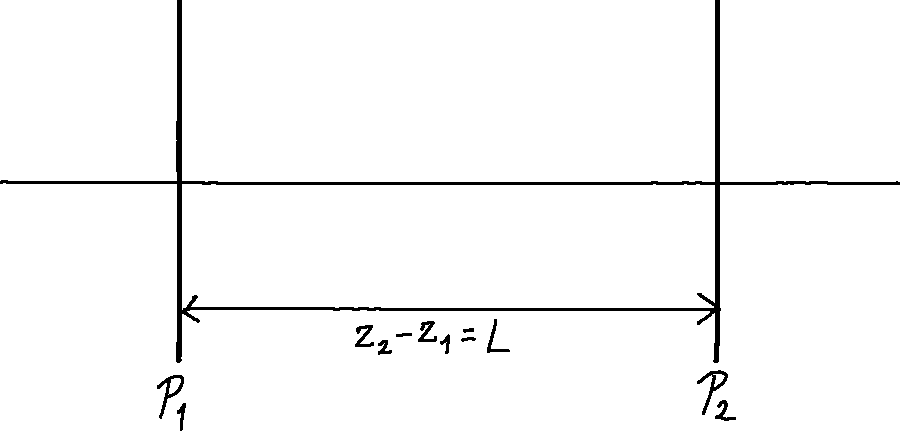
\includegraphics[width=.8\linewidth]{q2-setup}
	\end{figure}
	
	At $\mathcal{P}_1$, $E = 1/q_1 \mathrm{e}^{ikz_1} \mathrm{e}^{ik\rho_1^2 / 2q_1}$ where $\rho_1^2 = x_1^2 + y_1^2$.
	
	By Collins integral, we have:
	\begin{align*}
		E(\mathcal{P}_2) &= \frac{1}{i\lambda B} \int E \mathrm{ikl} \inftsml{x_1} \inftsml{y_1} \\
		&= \frac{1}{i\lambda B} \frac{\mathrm{e}^{ikz_1}}{q_1} \mathrm{e}^{ikl_0} \mathrm{e}^{ik/2B D(x_2^2 + y_2^2)} \int \mathrm{e}^{ik\rho_1^2/2q_1} \mathrm{e}^{ik/2B \sbracket{A(x_1^2 + y_1^2) - 2(x_1 x_2 + y_1 y_2)}} \inftsml{x_1} \inftsml{y_1}
	\end{align*}
	
	We further evaluate the integral: \textbf{\color{red}(TO CHECK)}
	\begin{align*}
		\int& \exp\cbracket{ik \sbracket{x_1^2 \rbracket{\frac{1}{2q_1} + \frac{A}{2B}} - x_1 \cdot \frac{2x_2}{2B} + y_1^2 \rbracket{\frac{1}{2q_1}} - y_1 \cdot \frac{2y_2}{2B}} \ldots}
	\end{align*}
	
	\part \todo Sketch of the setup again:
	\begin{figure}[H]
		\centering
		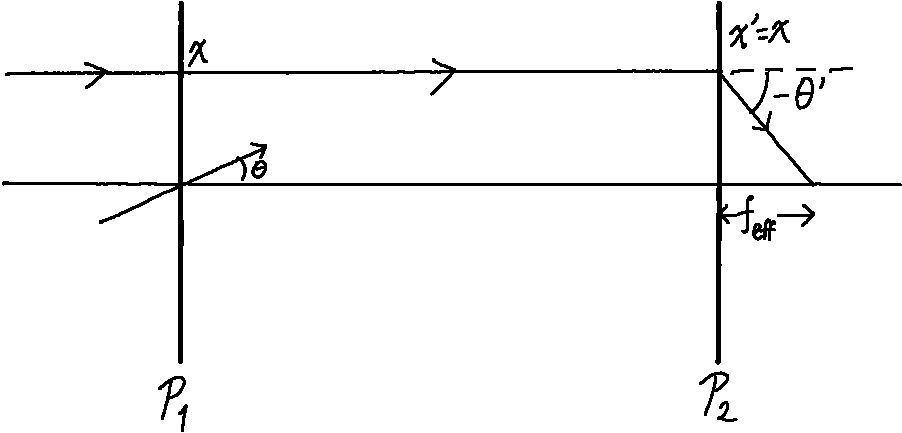
\includegraphics[width=.8\linewidth]{q2-setup-ray}
	\end{figure}
	
	Ray transfer matrix:
	???
	
	\part Ray transfer matrix for propagation over $f$ $\rightarrow$ lens $\rightarrow$ propagation over $f$:
	\begin{align*}
		\begin{pmatrix}
			1 & f \\
			0 & 1
		\end{pmatrix}
		\begin{pmatrix}
			1 & 0 \\
			-\frac{1}{f} & 1
		\end{pmatrix}
		\begin{pmatrix}
			1 & f \\
			0 & 1
		\end{pmatrix} &=
		\begin{pmatrix}
			1 & f \\
			0 & 1
		\end{pmatrix}
		\begin{pmatrix}
			1 & f \\
			-\frac{1}{f} & 0
		\end{pmatrix} \\
		&= \begin{pmatrix}
			0 & f \\
			-\frac{1}{f} 0
		\end{pmatrix}
	\end{align*}
	
	So $\mathcal{P}_1 \rightarrow \mathcal{P}_2$ has ray matrix:
	\begin{align*}
		\begin{pmatrix}
			0 & f \\
			-\frac{1}{f} & 0
		\end{pmatrix}
		\begin{pmatrix}
			0 & f \\
			-\frac{1}{f} 0
		\end{pmatrix}
		\begin{pmatrix}
			1 & d \\
			0 & 1
		\end{pmatrix}
		&= \begin{pmatrix}
			-1 & 0 \\
			0 & -1
		\end{pmatrix}
		\begin{pmatrix}
			1 & d \\
			0 & 1
		\end{pmatrix} \\
		&= \begin{pmatrix}
			-1 & -d \\
			0 & -1
		\end{pmatrix}
	\end{align*}
	
	So we have $l$:
	\begin{align*}
		l &= \rbracket{d + 4f} + \frac{1}{-2d} \sbracket{-(x_1^2 + y_1^2) - 2(x_1 x_2 + y_1 y_2) - (x_2^2 + y_2^2)}
	\end{align*}
	
	Note that compared to just propagating through $d$, $A$, $B$, and $D$ have all their signs flipped.
	
	For negative $d$, consider the system below:
	\begin{figure}[H]
		\centering
		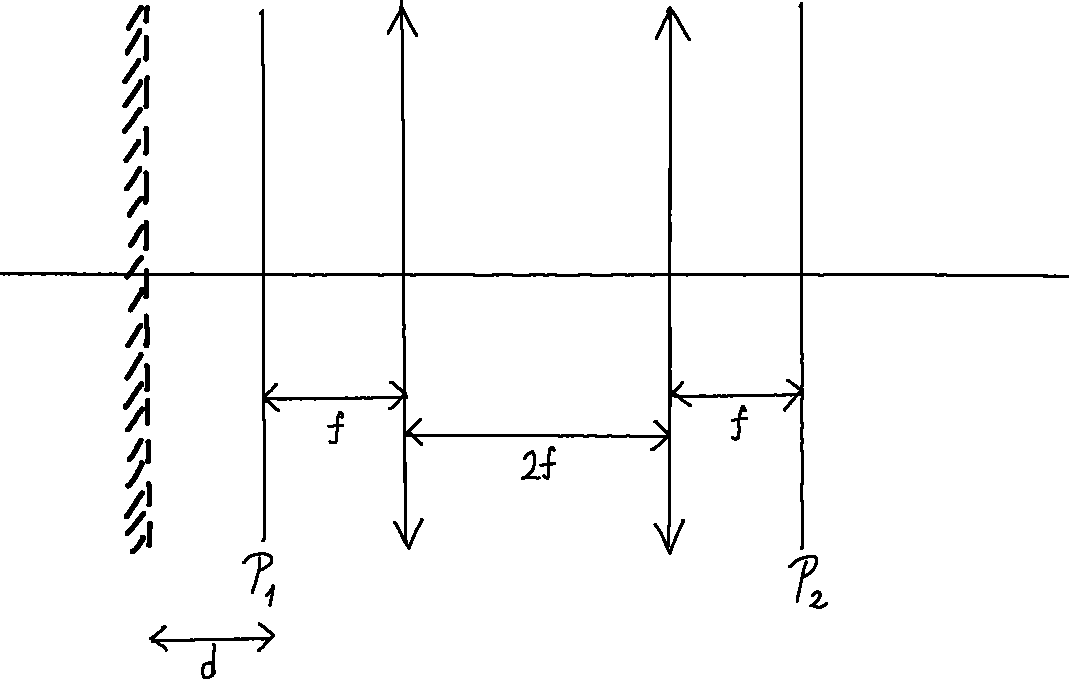
\includegraphics[width=.8\linewidth]{q2-negative-d}
	\end{figure}
	
	We have propagation by $|d|$ $\rightarrow$ reflect $\rightarrow$ ($f$ lens $f$):
	\begin{align*}
		\begin{pmatrix}
			-1 & 0 \\
			0 & -1
		\end{pmatrix}
		\begin{pmatrix}
			1 & 0 \\
			0 & -1
		\end{pmatrix}
		\begin{pmatrix}
			1 & |d| \\
			0 & 1
		\end{pmatrix} = ???
	\end{align*}
	
	So $B$ flips $\Rightarrow$ $l$ increases then decreases.
	
	\part Noting that $l$ may be adjusted to be positive or negative, thus this may be used to control dispersion in a CPA chain.
\end{parts}